\documentclass[a4paper,11pt]{article}

% Identificação
\newcommand{\pbtitulo}{OpenRefine}
\newcommand{\pbversao}{1.0}

\usepackage{../sty/tutorial}

%----------------------------------------------------------------------
% Início do Documento
%----------------------------------------------------------------------
\begin{document}
	
\maketitle % mostrar o título
\thispagestyle{fancy} % habilitar o cabeçalho/rodapé das páginas

%--------------------------------------------------------------------------
% RESUMO DO ARTIGO
%--------------------------------------------------------------------------
\begin{abstract}
  % O primeiro caractere deve vir com \initial{}
  \initial{O}\textbf{penRefine \cite{openrefineoficial} é um aplicativo gratuito e de código aberto para manipular todos os tipos de arquivos de dados. Escrito em linguagem Java, roda em qualquer sistema operacional através do navegador. Criado para obter rapidamente uma visão geral do conteúdo de um conjunto de dados, resolver inconsistências e aprimorá-lo com outros dados - tudo de maneira visual, interativa e eficiente. Pense nele como um editor de Planilhas voltado exclusivamente para o tratamento de dados.}
\end{abstract}

%--------------------------------------------------------------------------
% CONTEÚDO DO ARTIGO
%--------------------------------------------------------------------------
\section{Parte inicial}
Quase todos os conjuntos de dados que encontramos estão sujos e bagunçados. Existem inconsistências na maneira como os dados são inseridos - que vão desde erros de ortografia, duplicidades a espaços irregulares - que podem dificultar a análise posterior.

Limpar os dados é uma tarefa que leva um considerado tempo, mas tem que ser realizada de qualquer forma antes de tentar usá-los. \textbf{OpenRefine} nasceu com o objetivo de realizar esse trabalho sujo, realiza uma infinidade de tarefas para limpeza, organização e melhora da informação.
\begin{figure}[H]
	\centering
	
\includegraphics[width=0.5\textwidth]{imagem/logo.jpeg}
	\caption{Logo do OpenRefine}
\end{figure}

Mas tudo isso não poderia ser feito com o \textbf{MS-Excel} ou \textbf{Calc} (\textbf{LibreOffice})? Diria que talvez sim se sua massa for pequena, mas tente trabalhar com Gigas ou Teras de informação e verá que esses programas não lhe atenderão mais. Por ser extremamente leve e portátil, \textbf{OpenRefine} é a solução ideal para qualquer tipo de trabalho.

Seu início foi como um projeto chamado \textbf{Freebase Gridworks}, que foi comprado pela \textbf{Google} e reconstruído como \textbf{GoogleRefine} em 2010. O suporte oficial terminou em 2012 e houve uma transição para o projeto de código aberto denominado \textbf{OpenRefine}. Se olharmos bem \textbf{GoogleRefine} e \textbf{OpenRefine} é o mesmo aplicativo, muitos tutoriais e documentação usam os nomes de forma intercambiável. 

Casos que devemos usar: \vspace{-1em}
\begin{itemize}
	\item Limpeza - descobrir, corrigir inconsistências e agrupamentos.
	\item Transformar - alterar formatos, remodelar com divisão ou união de colunas com vários valores, transposição de colunas ou linhas.
	\item Estender - enriquecer os dados combinando-os a arquivos, mesclando projetos, buscando URLs ou com bancos de dados on-line.
	\item Automatizar - podemos reutilizar sua rotina de processamento exportando o histórico de operações em JSON e criar uma rotina programável.
\end{itemize}

Este é um programa extremamente flexível, qualquer formato tabular, tais como, planilhas, bancos de dados, XML, RDF, matrizes ou JSON pode ser visualizado. Além disso, foi projetado para ser extensível, a comunidade criou vários \textit{plugins} e extensões especializadas.

\textbf{OpenRefine} não apenas permite diagnosticar rapidamente a precisão de seus dados, mas também a agir em certos tipos de erros, muitas vezes de maneira automatizada. Podemos identificar facilmente erros sistemáticos, tais como, células em branco, duplicatas, inconsistências ortográficas entre outros. 

\section{OpenRefine no Docker}
Facilmente podemos obter o \textbf{OpenRefine} através do Docker. Criar uma pasta para associar ao contêiner onde colocaremos nossos dados: \\
\codigo{\$ mkdir \$HOME/openrefine\_home}

Fornecer permissões a pasta de modo que o contêiner possa acessá-la: \\
\codigo{\$ chown 1000 \$HOME/openrefine\_home}

Baixar a imagem disponível: \\
\codigo{\$ docker pull vimagick/openrefine}

Criar o container: \\
\codigo{\$ docker run -d --name meu-openrefine -p 3333:3333 -v \$HOME/openrefine\_home:/data:z vimagick/openrefine}

Para executar abrir um navegador e acessar a URL \url{http://localhost:3333}.

\subsection{Para atualizar o OpenRefine no Docker}
Quando existir uma nova versão disponível, podemos atualizar diretamente no contêiner do Docker. Contêiner possui um conceito de dinamicidade, ou seja, são atualizáveis e basicamente a única diferença é que devemos entrar nele para proceder isso.

Entrar no container: \\
\codigo{\$ docker exec -u 0 -it meu-openrefine bash}

Ir para o local correto: \\
\codigo{\$ cd /app}

Baixar e instalar: \\
\codigo{\$ set -xe \&\& apk add --no-cache bash curl tar \&\& curl -sSL https://github.com/ \\ OpenRefine/OpenRefine/releases/download/[versão]/openrefine-linux-[versão].tar.gz | tar xz --strip 1}

Sair do bash: \\
\codigo{\$ exit}

Reiniciar o container: \\
\codigo{\$ docker restart meu-openrefine}

E no navegador teremos a nova versão:
\begin{figure}[H]
	\centering
	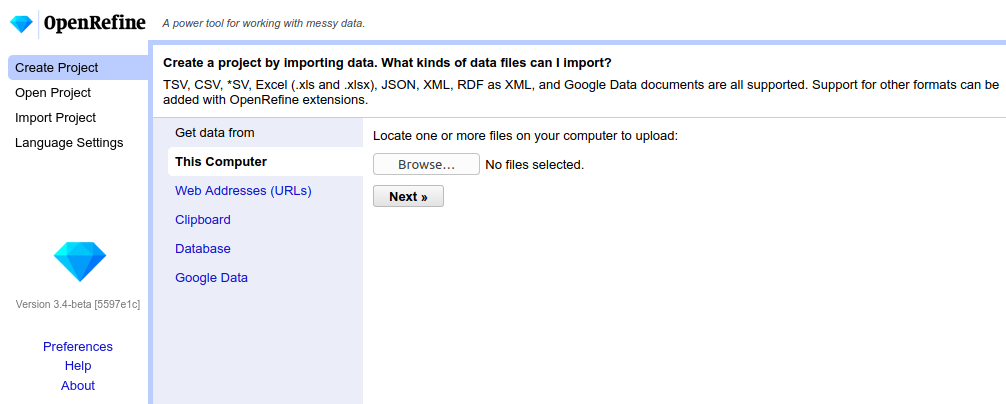
\includegraphics[width=0.8\textwidth]{imagem/novaVersao.png}
	\caption{Versão atual do OpenRefine}
\end{figure}

\section{Passos Iniciais}
No menu a esquerda temos as opções: \vspace{-1em}
\begin{itemize}
	\item \textbf{Criar um Projeto} - que permite importar uma base de dados de um arquivo ou de um banco que graças a linguagem Java podemos - através de uma conexão \textbf{JDBC} - utilizar qualquer banco de dados conhecido, buscá-la de um endereço Web que também (graças a sua passagem na Google) pode ser uma Planilha Google.
	\item \textbf{Abrir um Projeto} - uma vez criado, os projetos ficam a nossa disposição para reusá-los.
	\item \textbf{Importar um Projeto} - abrir um projeto criado por terceiros.
	\item \textbf{Escolher a linguagem} - pessoalmente prefiro mantê-lo em língua inglesa, mas se desejar pode optar pelo português.
\end{itemize}

Para os nossos exemplos vamos utilizar um arquivo chamado \textbf{marketSales.csv} que está disponibilizado em \url{https://github.com/fernandoans/machinelearning/tree/master/bases}. Baixar o arquivo, clicar em \opcmenu{Create Project } $\triangleright$ \opcmenu{This computer}. Pressionar \opcbotao{Browse}. Localizar o arquivo e no retorno pressionar \opcbotao{Next}.
\begin{figure}[H]
	\centering
	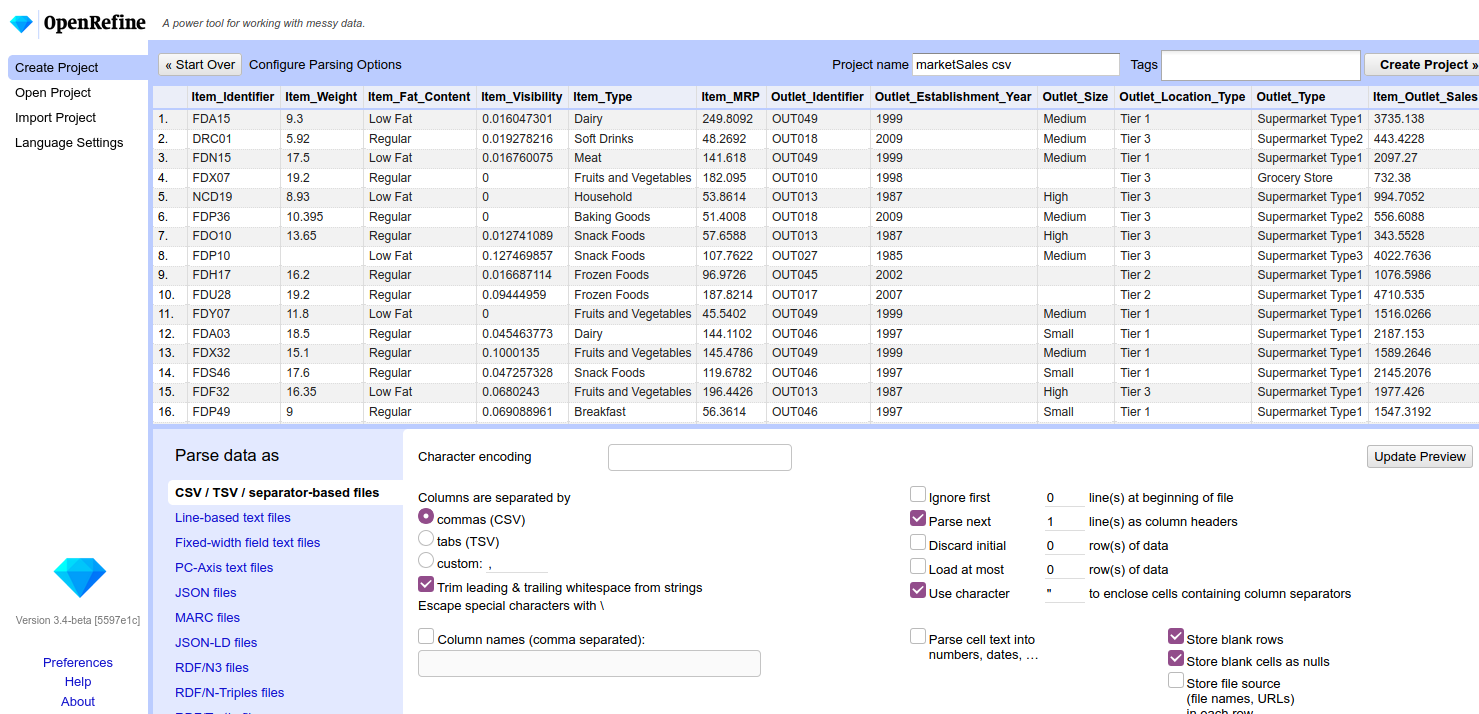
\includegraphics[width=0.8\textwidth]{imagem/dadosParaImportar.png}
	\caption{Dados para Importar}
\end{figure}

Essa janela é uma simples conferência de como o OpenRefine visualiza seus dados, podemos realizar os ajustes, caso haja necessidade, tais como, alterar o separador, a partir de qual linha começará a leitura, se linhas em branco devem ser consideradas ou não, o formato correto do arquivo (CSV, JSON, XML, XLS) entre muitas outras opções. Uma vez concluído pressionar \opcbotao{Create Project}.
\begin{figure}[H]
	\centering
	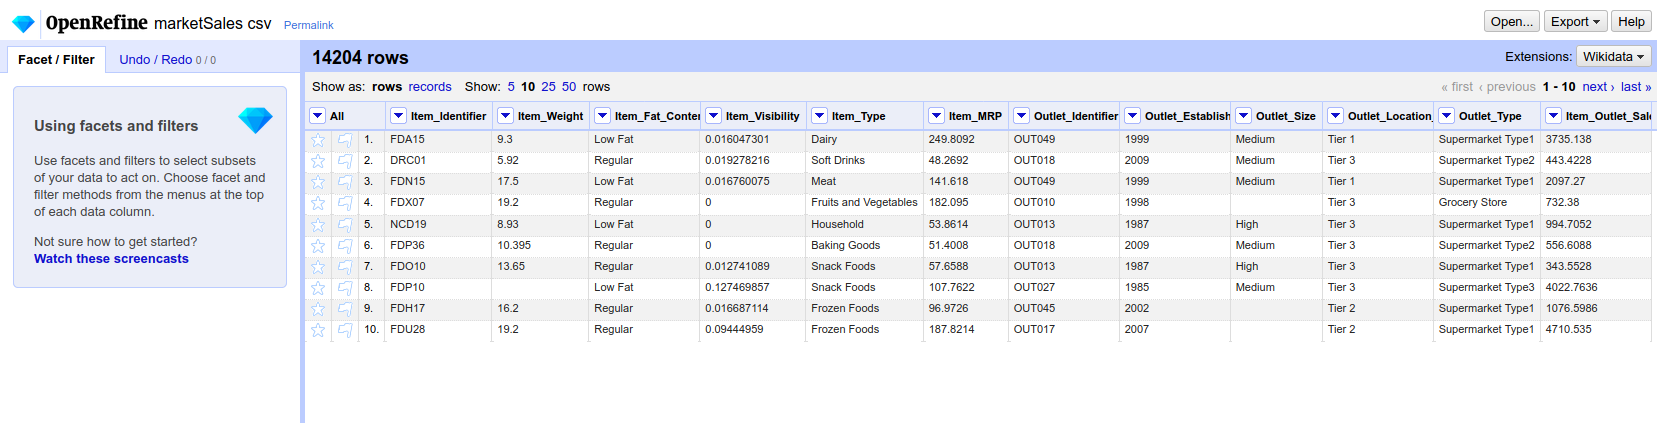
\includegraphics[width=0.8\textwidth]{imagem/projetoCriado.png}
	\caption{Dados Importados}
\end{figure}

Não devemos nos assustar uma vez que o ambiente de trabalho é o mesmo que qualquer planilha eletrônica, a exceção aqui é o conceito \textit{facet}. 

\subsection{Facets}
Isso seria algo como um filtro que é aplicado a cada coluna (ou a forma como a enxergaremos nossos dados - isso vem de \aspas{faceta} por essa palavra não ser comum adotaremos nesta apostila o termo FILTRO), são extremamente importantes para a visualização. Esses filtros uma vez criados são trabalhados na parte a esquerda. 

O tipo da coluna define a ela propriedades únicas, por exemplo duas colunas numéricas são unidas com operações matemáticas, já se forem caracteres muda para concatenação. Sendo assim vamos definir que para as colunas: \textbf{Item\_Weight}, \textbf{Item\_Visibility}, \textbf{Item\_MRP} e \textbf{Item\_Outlet\_Sales} o tipo numérico. Clicar $\bigtriangledown$ da coluna e selecionar \opcmenu{Edit Cells } $\triangleright$ \opcmenu{Common transforms } $\triangleright$ \opcmenu{To number}.

Errou alguma coluna? Não se desespere, isso aqui é como jogos de \textit{video game}, a cada ação é criado um ponto de controle, na aba \textit{Undo/Redo} (no menu a esquerda) podemos visualizar todas as ações que foram realizadas e a qualquer momento retornar a um ponto de mudança. Isso significa que iremos perder tudo o que fizemos? Depende, isso varia da quantidade de ações que retornamos. É como um histórico armazenado em memória.

As colunas modificadas ficaram na cor verde o que indica que são numéricas, vamos tentar abrir a coluna \textbf{Item\_Type} como um filtro numérico. Clicar $\bigtriangledown$ desta e selecionar \opcmenu{Facet } $\triangleright$ \opcmenu{Numeric Facet}. Obtemos uma janela de erro (no lado esquerdo) com a informação que esta coluna não possui esse tipo.

\begin{minipage}{\textwidth}
	\vspace{5pt}
	\begin{wrapfigure}{l}{0.25\textwidth}
		\vspace{-\baselineskip}
		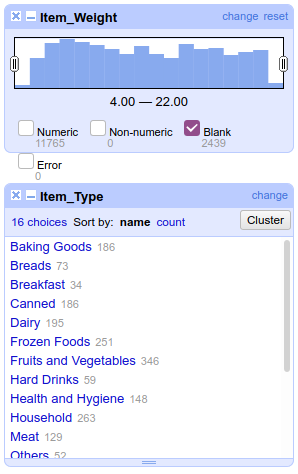
\includegraphics[width=0.9\linewidth]{imagem/facets.png} 
	\end{wrapfigure}
	Tentemos proceder de maneira similar em qualquer uma das colunas que definimos como numéricas. Na esquerda aparece um histograma com o que existe nessa coluna: quantidade de numéricos, não numéricos, brancos e erros. Se desmarcarmos ou marcamos qualquer opção esta ação é refletida na visão dos dados. \\[3mm]
	Para as tipo texto essa janela aparece de forma diferente, como um filtro de opções mostrando a quantidade de cada valor (fica horrível para uma coluna com valores únicos, como \textbf{Item\_Identifier}). Podemos ver isso aplicado corretamente. Clicar $\bigtriangledown$ de \textbf{Item\_Type} e selecionar \opcmenu{Facet } $\triangleright$ \opcmenu{Text Facet}. Serve para verificarmos como estão os dados, se existem nulos os discrepâncias. Também temos a possibilidade de abrir um histograma para este tipo, opção \opcmenu{Facet by choice counts } que aparece ao final da lista.
\end{minipage}

\subsection{Variáveis}
Antes de começarmos a ver qualquer coisa prática temos que ter a noção do que são variáveis para o \textbf{OpenRefine}, na verdade para o \textbf{GREL} (\textit{General Refine Expression Language}). Existem as básicas que são:
\begin{itemize}[nolistsep]
	\item \textit{row} - objeto contendo a linha atual.
	\item \textit{cell} - célula específica que está baseado em uma coluna da linha.
	\item \textit{value} - valor de uma determinada \textit{cell} ou \textit{record}, pode ser nulo.
\end{itemize}

Devemos nos atentar para que existe uma diferença entre \textit{cell} (célula) e \textit{column} (coluna). Podemos realizar ações para cada uma delas separadamente, por exemplo a função $split$ em célula significa criar várias colunas, já em coluna diversas linhas. A transformação (modificação do valor) ocorre na célula nunca na coluna.

\textit{Row} que se refere a linha atual, possui as seguintes propriedades:
\begin{itemize}[nolistsep]
	\item \textit{row.index} - índice de cada linha (inicia por 0).
	\item \textit{row.cells} - objeto contendo as células de uma linha.
	\item \textit{row.columnNames} - lista com o nome das colunas.
	\item \textit{row.starred} - indica se a linha está marcada com a estrela.
	\item \textit{row.flagged} - indica se a linha está marcada com a bandeira.
\end{itemize}

Por exemplo, as expressões: \\
\codigo{row.cells[\aspas{Item\_Type}].value \\
	cell.value}

Retornam exatamente o mesmo valor se estivermos na coluna \textbf{Item\_Type}, se estamos em outra e desejamos obter o valor de \textbf{Item\_Type} somente a primeira expressão serviria.

\textit{Rows} (linhas) e \textit{Records} são diferentes, mesmo que aparentem serem iguais, quando realizamos o \textit{split} em uma célula, provavelmente teremos mais linhas que registros, ou seja, o registro não muda. Por exemplo, na coluna \textbf{Outlet\_Type} desejamos saber quantos supermercados existem pouco importa seu tipo. Ao ativarmos \textit{text facet} veremos que temos 3 tipos, não é necessário fazer contas, vamos separar os valores. 

Clicar $\bigtriangledown$ de \textbf{Outlet\_Type} e selecionar \opcmenu{Edit cells } $\triangleright$ \opcmenu{Split multi-valued cells...}. Em \opcmenu{Separator } colocar um espaço em branco. E através de um filtro de texto vemos que são 12.399 supermercados. E na informação da janela principal são 28.408 linhas, se marcarmos \textbf{records} continuamos com os mesmos 14.204 registros. Ou seja, apenas a visão deles mudou.

\subsection{Ordenações}
A opção $\bigtriangledown$, além dos filtros, temos as possibilidades de ações que podemos proceder, como ordenar por exemplo. A partir do momento que ordenamos por determinada coluna esta se torna o padrão, a próxima coluna que procedemos a mesma ação vira uma espécie de segunda ordem, ou seja, uma ordenação dentro da outra. 

Vamos clarear esse conceito, ordenar numericamente \textbf{Item\_Visibility} (clicar $\bigtriangledown$ dessa e selecionar \opcmenu{Sort}, marcar a opção \opcmenu{smallest first}), em seguida ordenar de mesma forma a coluna \textbf{Item\_Height}. A ordem é: por \textbf{Item\_Visibility} e para cada valor repetido ordena por \textbf{Item\_Height}. Além disso, o \textbf{OpenRefine} corrigiu todos os menus, clicar $\bigtriangledown$ de \textbf{Item\_Visibility} e selecionar \opcmenu{Sort } que agora possui mais possibilidades como \opcmenu{Reverse } (inverter a ordenação) ou \opcmenu{Remove Sort } (remover esta ordenação). Além disso, acima da planilha de dados aparece a opção \opcmenu{Sort } que possui as seguintes opções: \opcmenu{Remove Sort } (remover todas as ordenações), \opcmenu{Reorder rows permanently } (aplicar esta ordenação de forma permanente) e as opções para cada coluna na ordem que aparecem no filtro.

\subsection{Duplicados}
Não é o caso de nenhuma coluna neste conjunto, mas vamos imaginar que uma delas deveria ser a chave primária da coleção, ou seja, conter apenas valores únicos, como saber se nela existem termos duplicados? Clicar $\bigtriangledown$ da coluna e selecionar \opcmenu{Facet } $\triangleright$ \opcmenu{Customized facets } $\triangleright$ \opcmenu{Facet by blank } é mostrado dois valores \textit{true} (linhas que contém valores duplicados) e \textit{false} (que não contém), ou seja, basta clicarmos em \textit{true} e veremos que linhas são essas para arrumarmos.

\section{Limpeza dos Dados}
Para praticarmos um pouco feche este projeto (clicar no símbolo do OpenRefine no canto superior esquerdo) baixar e abrir a planilha \textbf{LouisianaSecretaryOfStateOfficials.xls} (disponibilizado no mesmo endereço do GitHub). Essa contém os dados dos Funcionários da Secretaria do Estado de Louisiana nos EUA.

Nossa primeira preocupação é transformar corretamente os dados, para as colunas \textbf{Expiration Date} e \textbf{Commissioned Date} devemos transformar para data. Clicar $\bigtriangledown$ de cada coluna e selecionar \opcmenu{Edit Cells } $\triangleright$ \opcmenu{Common transforms } $\triangleright$ \opcmenu{To date}. Agora podemos aplicar para essa o \textit{timeline facet}.

Aplicar aos seguintes filtros: \vspace{-1em}
\begin{itemize}
	\item \textit{timeline facet} das colunas \textbf{Expiration Date} e \textbf{Commissioned Date} marcar somente a opção \opcmenu{Blank}
	\item \textit{text facet} das colunas \textbf{Candidate Name} e \textbf{Office Phone} marcar a opção \opcmenu{Blank}.
\end{itemize}

Existem 901 registros a serem descartados pois não contém nenhuma informação essencial.
\begin{figure}[H]
	\centering
	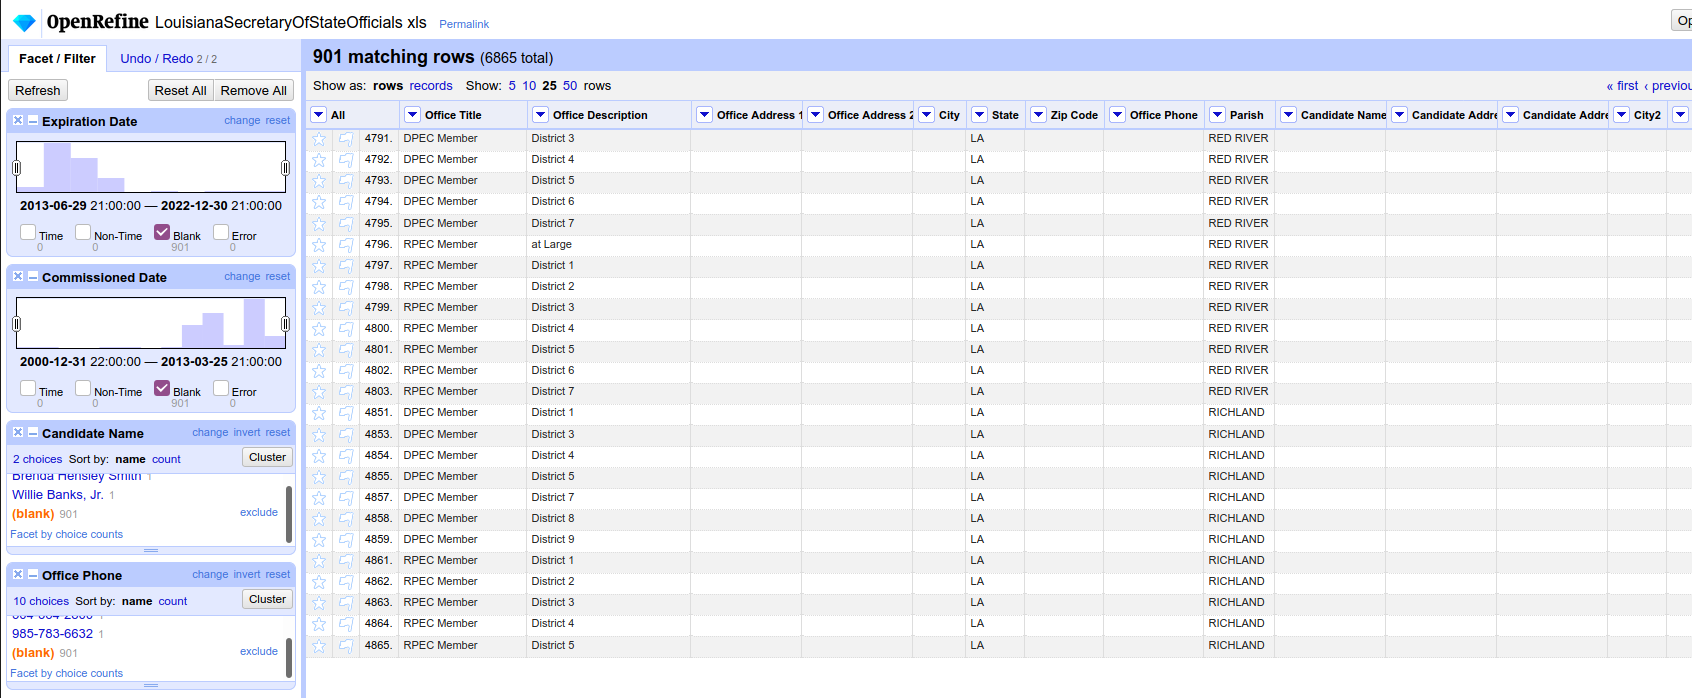
\includegraphics[width=0.7\textwidth]{imagem/limpeza1.png}
	\caption{Filtros aplicados}
\end{figure}

São descartáveis pois não contém qualquer informação que pode nos auxiliar no seu preenchimento, por exemplo sabemos que temos o título, a descrição do escritório (alguns tem até a paróquia), porém sem o nome, telefone e datas do cargo não temos como saber quem são.

Para eliminá-los, clicar $\bigtriangledown$ da primeira coluna e selecionar \opcmenu{Edit Rows } $\triangleright$ \opcmenu{Remove matching rows}. Se desejar eliminar todos selecionar \opcmenu{Remove All } de \textit{Facet/Filter} (no lado superior esquerdo).

\subsection{Outro tipo de duplicados}
Um tipo mais comum de registros duplicados é quando eles não se batem por alguma diferença, por exemplo, maiúsculas e minúsculas, zero na frente, mesma palavra mas escrita com grafia diferente. 

\begin{minipage}{\textwidth}
	\vspace{5pt}
	\begin{wrapfigure}{l}{0.25\textwidth}
		\vspace{-\baselineskip}
		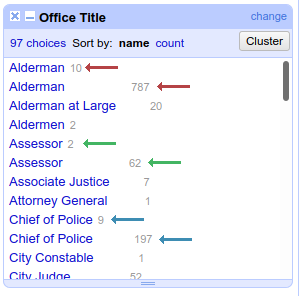
\includegraphics[width=0.9\linewidth]{imagem/duplicados.png} 
	\end{wrapfigure}
	Por exemplo, aplicar o \textit{text facet} na coluna \textbf{Office Title} e vemos que existem vários títulos nessas condições. \\[3mm]
	Neste caso devemos ter cuidado pois é muito fácil tratá-los com o OpenRefine, ao nos posicionarmos que qualquer palavra do filtro (por exemplo, em \textit{Alderman}) aparece as opçoes \opcmenu{Edit } e \opcmenu{Include}. A primeira serve para modificar os registros e a segunda para mostrá-los na janela principal.
\end{minipage}

Para procedermos a alteração, selecionamos o segundo \textit{Alderman} e pressionamos a opção \opcmenu{Edit } observamos que existem espaços ao final da palavra, retirar e pressionar \opcbotao{Apply}.
\begin{figure}[H]
	\centering
	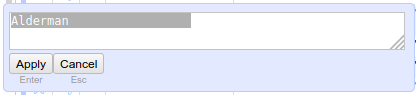
\includegraphics[width=0.4\textwidth]{imagem/duplicados2.png}
	\caption{Opção de Edição}
\end{figure}

Porém essa forma só é aplicada quanto a grafia diferente, mudar os títulos \textit{Alderman at large} e \textit{Aldermen} para \textit{Alderman} da mesma forma. Quando temos muitas informações na mesma situação, por exemplo remover espaços, ao invés de editar cada uma podemos aplicar a função $trim$ (elimina os espaços em branco tanto da direita quanto da esquerda) e eliminar todos de uma só vez.

Clicar $\bigtriangledown$ de \textbf{Office Title} e selecionar \opcmenu{Edit Cells } $\triangleright$ \opcmenu{Common transforms } $\triangleright$ \opcmenu{Trim leading and trailing whitespace}. Assim todos com esse tipo de duplicidade se resolvem.

Outra forma de vermos os duplicados é aplicando a técnica de \textbf{clusterização}, esta localiza automaticamente os semelhantes e os agrupa. Clicar $\bigtriangledown$ de \textbf{Office Title} e selecionar \opcmenu{Edit Cells } $\triangleright$ \textbf{Cluster and Edit}. Na janela \textit{Cluster \& Edit} alterar \opcmenu{Method } para \textit{nearest neighbor}.
\begin{figure}[H]
	\centering
	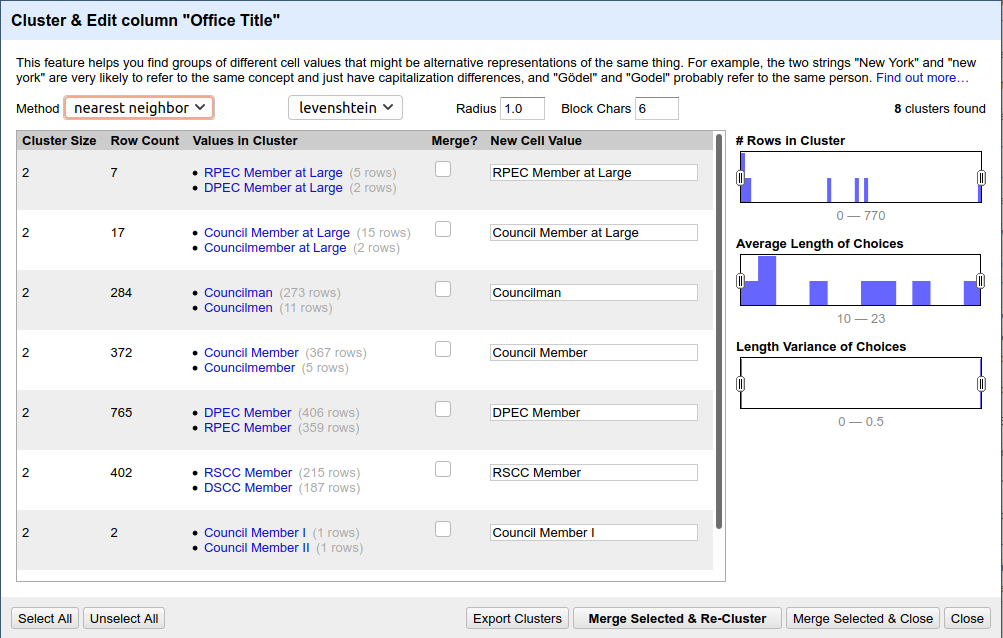
\includegraphics[width=0.7\textwidth]{imagem/cluster.png}
	\caption{Clusterização e Edição}
\end{figure}

Outra forma de lidarmos com esses duplicados é através de uma troca (Replace) direta, por exemplo, alguns títulos possuem a palavra \textit{at large} ao final. Clicar $\bigtriangledown$ de \textbf{Office Title} e selecionar \opcmenu{Edit Cells } $\triangleright$ \opcmenu{Replace}. Em \opcmenu{find } digitar \aspas{ at large} (sem as aspas e com o espaço) e marcar \opcmenu{case insensitive}. Não colocar nada em \opcmenu{Replace with}. Pressionar \opcbotao{OK}. Outro caso é com o texto \aspas{(s)} que aparece em alguns títulos, realizar a troca de mesma forma para praticar.

Algumas realmente não existirá forma a não ser realizarmos a edição da maneira como foi mostrado no início dessa sessão, como por exemplo o título \textit{Councilmember} que aparece junto e deve ser trocado para \aspas{Council Member}. Mas mesmo assim, observamos que o OpenRefine torna fácil o trabalho de lidar com duplicados.

\subsection{Separar Informação}
Vamos pegar um caso curioso que acontece com a coluna \textbf{Office Address}, muitos endereços são fornecidos apenas como uma caixa postal (P.O. Box), então vamos criar uma nova coluna que conterá essa informação. Primeiro usar as técnicas aprendidas para deixar todas as caixas postais com o formato correto: \aspas{P.O. Box} (sem aspas). Algumas estão muito separadas e outras muito juntas. E ainda existe o caso que ao invés de \textit{Box} está escrito \aspas{Drawer} (gaveta).

Uma vez que temos todas em um padrão único. Podemos criar um filtro para nos mostrar as que possuem ou não \aspas{P.O. Box} sem termos o trabalho de fazer essa ação a cada uma. Clicar $\bigtriangledown$ de \textbf{Office Address} e selecionar \opcmenu{Facet } $\triangleright$ \opcmenu{Custom text facet...}. 
\begin{figure}[H]
	\centering
	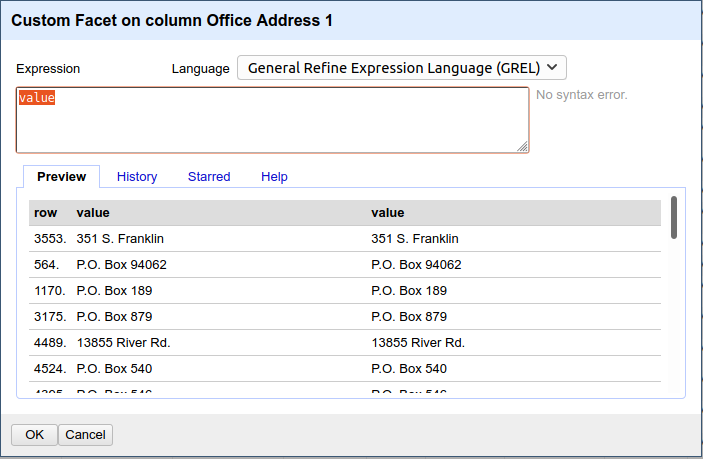
\includegraphics[width=0.6\textwidth]{imagem/customFacet.png}
	\caption{Filtro Customizado}
\end{figure}

Agora precisamos de conhecimento em \textbf{GREL}, não se preocupe tanto pois também podemos usar \textbf{Python} ou \textbf{Cloujure}. GREL é uma linguagem de Script bem simples de aprender, por exemplo para fazer o que desejamos basta escrever na caixa a expressão: \\
\codigo{value.startsWith(\aspas{P.O. Box})}

A função $startsWith$ (sua contrária é \textit{endsWith}) verifica se o valor inicia com um texto definido entre os parênteses. E ao pressionar \opcbotao{OK } teremos nosso filtro construído. Neste selecione a opção \textit{true}. 

Para criar a nova coluna. Clicar $\bigtriangledown$ de \textbf{Office Address} e selecionar \opcmenu{Edit column } $\triangleright$ \opcmenu{Add column based on this column...}. Informar o nome da coluna como \textbf{P.O. Box}. E a expressão em GREL: \\
\codigo{value.split(\aspas{ })[2]}

A função $split$ quebra o texto em várias partes, a primeira (índice 0) é \aspas{P.O.}, a segunda (índice 1) é \aspas{Box} e a terceira (índice 2) é a que nos interessa pois contém o valor da caixa postal. 

Como última troca vamos remover o número. Clicar $\bigtriangledown$ de \textbf{Office Address} e selecionar \opcmenu{Edit cells } $\triangleright$ \opcmenu{Transform}. E a expressão em GREL: \\
\codigo{value.split(\aspas{ })[0]+\aspas{ }+value.split(\aspas{ })[1]}

Aplicamos a mesma função $split$ porém obtendo as duas primeira palavras. E ao liberar o filtro, notamos que apenas os registros que continham a palavra \aspas{P.O. Box} ganharam seu número em uma nova coluna e este foi retirado da anterior. E temos 2.991 Secretários recebem sua correspondência por meio de Caixa Postal.

\subsection{Dependência de Informação}
Algo que acontece muito em limpeza de dados são informações conflitantes, por exemplo, acionar dois \textit{facet text} para as colunas \textbf{City} e \textbf{Zip Code}. O prefixo do código postal de uma cidade deve ser único, se selecionamos \textit{Alexandria} vemos que tem 3 prefixos diferentes: 71302 (com 1 registro), 71303 (com 2 registros) e 71309 (com 33 registros). 

Outro caso é parte de informação faltante, por exemplo, para o mesmo filtro desmarque a cidade e aparece um código postal com o valor 1022. Poderíamos chegar a uma conclusão errada que falta um \aspas{7} na frente (visto que a maioria dos valores iniciam com 7). Porém se selecionamos este veremos que sua cidade é \textit{Independence}, então desmarcamos este filtro e selecionamos esta cidade e vemos que os outros registros possuem o prefixo com valor \aspas{70443}.

Existem outras três colunas que também são dependentes: \textbf{Candidate Name}, \textbf{Sex} e \textbf{Salutation}. porém para vê-las (sem ter que ficar indo de cá para lá na planilha) vamos \aspas{encolher} as colunas que não nos interessa. Clicar $\bigtriangledown$ de \textbf{Office Description} e selecionar \opcmenu{View } $\triangleright$ \opcmenu{Collapse this column}. E dessa forma conseguimos obter a visão das colunas que nos interessa. Para voltar ao tamanho padrão basta clicar na coluna fechada.
\begin{figure}[H]
	\centering
	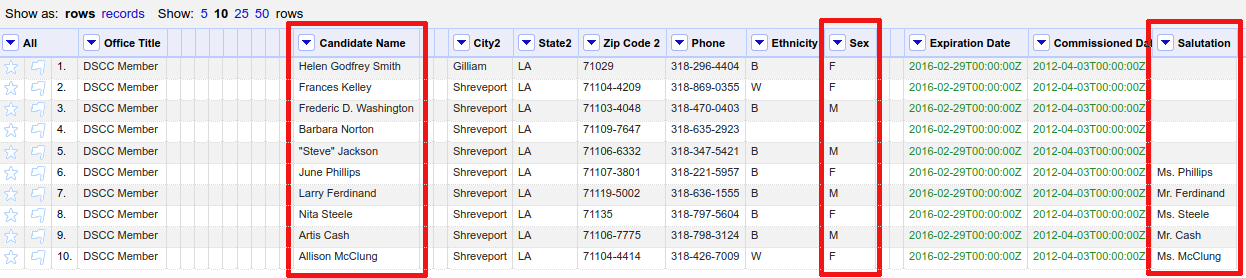
\includegraphics[width=0.8\textwidth]{imagem/colunasEncolhidas.png}
	\caption{Visão das Colunas de Interesse}
\end{figure}

Também podemos expandir ou encolher todas as colunas de uma só vez. Clicar $\bigtriangledown$ da primeira coluna \textbf{All} e selecionar \opcmenu{View}. Existem as seguintes opções:
\begin{itemize}[nolistsep]
	\item \textit{Collapse all columns} - encolher todas as colunas.
	\item \textit{Expand all columns} - espandir todas as colunas.
	\item \textit{Show/Hide 'null' values in cells} - mostrar ou esconder células com valores nulos.
\end{itemize}	
	
Devemos preencher os dados faltantes da coluna \textbf{Salutation} da seguinte forma: O pronome de tratamento (Mr. para \textbf{Sex} igual a \aspas{M} e Mrs. igual a \aspas{F}) seguido do último nome. Nosso primeiro problema é na coluna \textbf{Sex} no qual pode conter informação vazia, aplicar (conforme já mostrado) a função $trim$ que elimina os espaços em branco nesta coluna.

Próximo passo é criar um filtro para isolarmos somente os registros faltantes. Clicar $\bigtriangledown$ de \textbf{Salutation} e selecionar \opcmenu{Facet } $\triangleright$ \opcmenu{Customize facets } $\triangleright$ \opcmenu{Facet by null}. Aplicar o mesmo filtro para a coluna \textbf{Candidate Name}. Proceder de mesma forma para a coluna \textbf{Sex} porém usando a opção \opcmenu{Facet by empty string}.

Agora temos 3 filtros: marcar \opcmenu{true } para o filtro \textbf{Salutation} e \opcmenu{false } para \textbf{Candidate Name} e \textbf{Sex}. Nossa visão está restrita aos 1.773 registros que possuem nome e gênero mas não a forma de tratamento.

Precisamos criar uma coluna que contenha o pronome de tratamento devido com o último nome, devemos tomar cuidado pois esse pode conter Jr, III ou seja um sufixo de família. O nome anterior indica isso pois possui uma vírgula.

Clicar $\bigtriangledown$ de \textbf{Salutation} e selecionar \opcmenu{Edit cells } $\triangleright$ \opcmenu{Transform}. E a expressão em GREL: \\
\codigo{cells[\aspas{Sex}].value.replace(\aspas{M},\aspas{Mr. }).replace(\aspas{F},\aspas{Mrs. }) + \\ 
	cells[\aspas{Candidate Name}].value.split(\aspas{,})[-2].split(\aspas{ })[-1].trim()}

Primeiro a partir do gênero montamos se será \aspas{Mr.} ou \aspas{Mrs.}, na segunda parte usamos uma função $split$ para isolar o nome de família e uma segunda para obter o último nome. Ou seja, com uma única linha resolvemos nosso problema. O valor negativo para o índice trabalha de trás para frente neste, ou seja, valor -1 corresponde ao último valor, -2 ao penúltimo e assim sucessivamente. Pressionar \opcbotao{OK}. E remover os filtros.

\section{Funções do GREL}
Existem funções bem interessantes para se usar com o GREL, vejamos algumas que podem ser bem úteis para outros casos de limpeza.

\codigo{if (condição, caso Verdadeiro, caso Falso)}

Esse comando só serve para criamos uma nova coluna, por exemplo, \textbf{Salutation Complete} criada a partir da coluna \textbf{Sex} com a expressão: \\
\codigo{if(value.contains(\aspas{M}), \aspas{Mr. }, \aspas{Mrs. }) + \\ 
	cells[\aspas{Candidate Name}].value.split(\aspas{,})[-2].split(\aspas{ })[-1].trim()}

Esta função deve ser usada na coluna de origem, isso é \textbf{Sex}, e não em \textbf{Candidate Name}, pois senão retornaria errado. Como condicionais podemos usar:
\begin{itemize}[nolistsep]
	\item \textit{isBlank(valor)} - se o valor é vazio.
	\item \textit{isNonBlank(valor)} - se o valor não é vazio.
	\item \textit{isNull(valor)} - se o valor é nulo.
	\item \textit{isNotNull(valor)} - se o valor não é nulo.
	\item \textit{isNumeric(valor)} - se o valor não é numérico.
	\item \textit{isError(expressão)} - se a expressão retorna um erro.
	\item \textit{contains(valor)} - contém um determinado valor ou expressão.
	\item \textit{match(valor)} - é exatamente o valor ou expressão.
\end{itemize}

\codigo{diff(data final, data inicial, período)}

Temos duas datas em questão \textbf{Expiration Date} e \textbf{Commissioned Date}, a primeira corresponde ao dia de término do mandato e a outra seu início, se precisamos criar uma outra coluna com a diferença em dias. Clicar $\bigtriangledown$ de \textbf{Commissioned Date} e selecionar \opcmenu{Edit collumn } $\triangleright$ \opcmenu{Add column based on this column...}. E a expressão em GREL: \\
\codigo{diff(cells['Expiration Date'].value, value, \aspas{days})}

Para o perído podemos usar para esta diferença:
\begin{itemize}[nolistsep]
	\item \textit{minutes} - em minutos
	\item \textit{hours} - em horas
	\item \textit{days} - em dias
	\item \textit{months} - em meses
	\item \textit{years} - em anos
\end{itemize}

\codigo{row.index}

Esta função é útil quando necessitamos de uma chave primária, por exemplo, precisamos exportar os dados para uma tabela porém não existe nenhum campo que é candidato a ser a chave única, então basta escolher qualquer coluna e adicionar uma nova com a expressão: \\
\codigo{row.index + 1}

\codigo{with(avaliação, variável, expressão)}

Coloca o resultado da avaliação na variável e assim podemos simplificar a expressão a ser usada. Por exemplo, necessitamos criar uma coluna contendo o último nome do Funcionário (lembrar das regras). E a expressão em GREL: \\
\codigo{with(value.split(\aspas{,})[-2], a, a.split(\aspas{ })[-1])}

Temos as seguintes expressões matemáticas em GREL:
\begin{itemize}[nolistsep]
	\item \textit{floor(num)} - causa o arredondamento para baixo, $floor(3.9) = 3$
	\item \textit{ceil(num)} - causa o arredondamento para cima, $ceil(3.2) = 4$
	\item \textit{round(num)} - faz o arredondamento da forma padrão, $round(3.7) = 4$
	\item \textit{min(num1, num2)} - menor valor entre dois números.
	\item \textit{max(num1, num2)} - maior valor entre dois números.
	\item \textit{mod(num1, num2)} - módulo entre dois números. Ideal para sabermos quando o número é par, mod(num\_par, 2) é sempre igual a 0. Também quando é um múltiplo de outro valor $mod(9, 3) = 0$
	\item \textit{ln(num)} - logaritmo natural do número.
	\item \textit{log(num)} - logaritmo na base 10 do número.
	\item \textit{exp(num)} - exponencial do número.
	\item \textit{pow(base, expoente)} - base elevada ao expoente. A partir dessa podemos tirar a raiz quadrada elevando o número a 0.5, $pow(49, 0.5) = 7$
	\item \textit{sum(lista)} - somatório dos números, $sum([3, 4, 8, 7, 9]) = 31$
\end{itemize}

Não confundir, se estamos usando um valor definido (i.e \textbf{value} para criar uma nova coluna) então a função $floor$ é usada da seguinte maneira $value.floor()$, sem nenhum parâmetro, porém também podemos usá-la $floor(value)$. A mesma regra se aplica a qualquer outra função.

\codigo{filter(lista, variável, expressão)}

É ideal quando temos um lista de valores e queremos reduzir esta, somente para entendermos, temos valores contendo 3 possibilidades \aspas{Sr}, \aspas{Sr.} e \aspas{Senhor} queremos deixar somente o \aspas{Sr.}. Aplicamos a expressão em GREL: \\
\codigo{filter([\aspas{Sr}, \aspas{Sr.}, \aspas{Senhor}], v, v.length() == 3)}

Podemos ter as seguintes expressões de texto em GREL (a posição do primeiro caractere de um texto é 0):
\begin{itemize}[nolistsep]
	\item \textit{replace(val1, val2)} - troca um valor por outro.
	\item \textit{replaceChars(val1, val2)} - troca uma cadeia de caracteres por outra, é útil quando temos \aspas{sujeira} nos campos texto.
	\item \textit{startsWith(val)} - se o texto inicia por determinado valor.
	\item \textit{endsWith(val)} - se o texto termina por determinado valor.
	\item \textit{toString()} - transforma o valor para texto.
	\item \textit{indexOf(val)} - posição do texto para o valor informado, retorna -1 se não existir.
	\item \textit{lastIndexOf(val)} - posição do texto para o valor informado porém conta de trás para frente, retorna -1 se não existir.
	\item \textit{toLowercase()} - texto em minúsculas.
	\item \textit{toUppercase()} - texto em maiúsculas.	
	\item \textit{toTitlecase()} - início de cada palavra em maiúscula, ideal para corrigir nomes.	
	\item \textit{chomp(val)} - corta o termo final do texto se for similar ao valor.
	\item \textit{substring(inicial, final)} - corta um texto. O \textbf{final} é opcional mas se passado não será incluído, $substring(\aspas{Fernando},3) = \aspas{nando}$, porém $substring(\aspas{Fernando},3,6) = \aspas{nan}$
	\item \textit{splitByLengths(val1, val2, ...)} - transforma o texto em uma lista sendo que cada elemento tem seu tamanho definido.
\end{itemize}

\codigo{find(expressão)}

Se determinada expressão for encontrada no texto então esta será retornada, por exemplo, será que um determinado campo contém vogais? E como estas aparecem? Usamos a expressão: \\
\codigo{value.toLowercase().find(/[aeiou]+/).sort()}

Retorna uma lista com todas as vogais da expressão ordenadas alfabeticamente. Podemos ter as seguintes expressões de lista em GREL, normalmente algumas delas também podem ser aplicadas a texto:
\begin{itemize}[nolistsep]
	\item \textit{length()} - quantidade de elementos.
	\item \textit{sort()} - ordenar uma lista, numérica ou não.
\end{itemize}

\codigo{forEach(lista, variável, expressão)}
	
Avalia a lista, colocando cada valor na variável e chamando a expressão.

Possui algumas funções similares:
\begin{itemize}[nolistsep]
	\item \textit{forEachIndex(lista, índice, variável, expressão)} - além do valor passa o índice.
	\item \textit{forRange(início, fim, passo, variável, expressão)} - ao invés de usar uma lista de valores cria um laço com um valor inicial e final percorrendo os elementos conforme o passo.
	\item \textit{forNonBlank(lista, variável, expressãoNãoVazios, expressãoVazios)} - verifica se a variável em questão não é vazia e chama a primeira expressão, caso contrário a segunda.
\end{itemize}

Uma última função antes de terminarmos, para criarmos uma coluna com TODOS os valores das outras colunas? Use a expressão (que pode ser colocada na opção \opcmenu{Add column based on this column... } em qualquer coluna): \\
\codigo{forEach(row.columnNames,cn,cells[cn].value).join(\aspas{|})}

Acabou? Recomendo que veja o tutorial sobre Limpeza de Dados de \textbf{John Little} que está disponível no endereço \url{https://libjohn.github.io/openrefine/} e o blog \textbf{Open Refine for Librarians} em \url{http://liwong.blogspot.com/}. Sempre que tenho dúvidas recorro a ambos.
	
\section{Conclusão}
Como vimos os casos de uso do OpenRefine mostra que, como os pesquisadores, podemos diagnosticar e agir com base na precisão dos dados. Vimos os princípios e práticas da limpeza de dados, bem como o OpenRefine pode ser usado para executar tarefas essenciais que nos ajudam a obter o melhor dos dados.

Registros duplicados, valores vazios e formatos inconsistentes são fenômenos com os quais devemos estar preparados para lidar ao usar quaisquer conjuntos de dados. Levamos muito tempo para descobrir inconsistências nos dados contidos em uma simples planilha ou banco de dados. À medida que cada vez mais compartilhamos, agregamos e reutilizamos dados da Web, e devemos estar atentos a questões de qualidade de dados que inevitavelmente surgem.

Sou um entusiasta do mundo \textbf{Open Source} e novas tecnologias. Qual a diferença entre Livre e Open Source? \underline{Livre} significa que esta apostila é gratuita e pode ser compartilhada a vontade. \underline{Open Source} além de livre todos os arquivos que permitem a geração desta (chamados de arquivos fontes) devem ser disponibilizados para que qualquer pessoa possa modificar ao seu prazer, gerar novas, complementar ou fazer o que quiser. Os fontes da apostila (que foi produzida com o LaTex) está disponibilizado no GitHub \cite{github}. Veja ainda outros artigos que publico sobre tecnologia através do meu Blog Oficial \cite{fernandoanselmo}.

%--------------------------------------------------------------------------
% REFERÊNCIAS
%--------------------------------------------------------------------------
\begin{thebibliography}{4}
  \bibitem{openrefineoficial} 
  Página Oficial do OpenRefine \\
  \url{https://openrefine.org/}
  
  	\bibitem{fernandoanselmo} 
	Fernando Anselmo - Blog Oficial de Tecnologia \\
	\url{http://www.fernandoanselmo.blogspot.com.br/}
	
	\bibitem{publicacao} 
	Encontre essa e outras publicações em \\
	\url{https://cetrex.academia.edu/FernandoAnselmo}
	
	\bibitem{github} 
	Repositório para os fontes da apostila \\
	\url{https://github.com/fernandoans/publicacoes}
\end{thebibliography}
  
\end{document}
